
\documentclass[compress]{beamer}

\mode<presentation> {

    \usetheme{default}
    \useoutertheme{seb}
    \useinnertheme{seb}
% \usefonttheme{seb}
%\useoutertheme[subsection=false]{smoothbars} 


    \setbeamertemplate{navigation symbols}{} 
}
\usepackage{graphicx} 
\usepackage{booktabs}
\usepackage{amssymb} 

%----------------------------------------------------------------------------------------
%	TITLE PAGE
%----------------------------------------------------------------------------------------

\title{MCMC Diagnostics}

% \author{Helen Johnson}
\date{}

\begin{document}

    \begin{frame}
        \titlepage
    \end{frame}

\section{MCMC in practice}
\label{sec-8}
\begin{frame}[label=sec-8-1]{Review}
    In the practical you used \textit{Metropolis-Hastings} with a \textit{Gaussian} proposal distribution to infer \textit{one} parameter, $R_0$\\~\\

    In this session we will:
    \begin{itemize}
        \item extend to multivariate inference
        \item learn about MCMC diagnostics
        \item think about accuracy and efficiency
    \end{itemize}
\end{frame}

\begin{frame}[label=sec-8-2]{Interlude: Multivariate Gaussian distribution}
    To infer more multiple parameters we can use multivariate Gaussian\\~\\
    \begin{columns}[c] 
    \column{.5\textwidth} 
    mean $\mu = \begin{bmatrix} 3 & 2 \end{bmatrix}$\\
    covariance $\Sigma =  \begin{bmatrix} 25 & 0 \\ 0 & 9 \end{bmatrix}$
    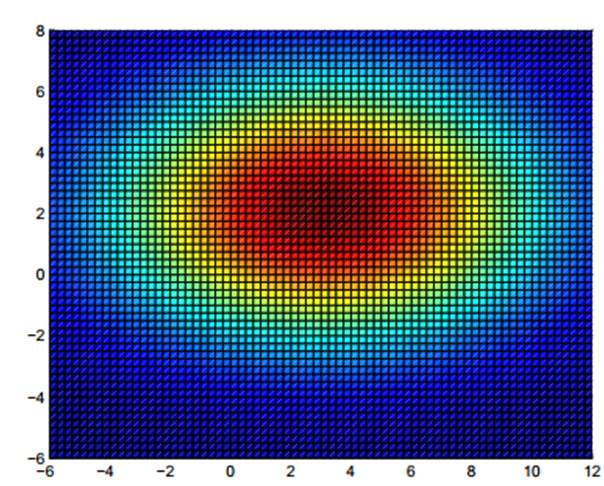
\includegraphics[width=0.8\linewidth]{MVN1}

    \column{.5\textwidth}
    mean $\mu = \begin{bmatrix} 3 & 2 \end{bmatrix}$\\
    covariance $\Sigma =  \begin{bmatrix} 10 & 5 \\ 5 & 5 \end{bmatrix}$
    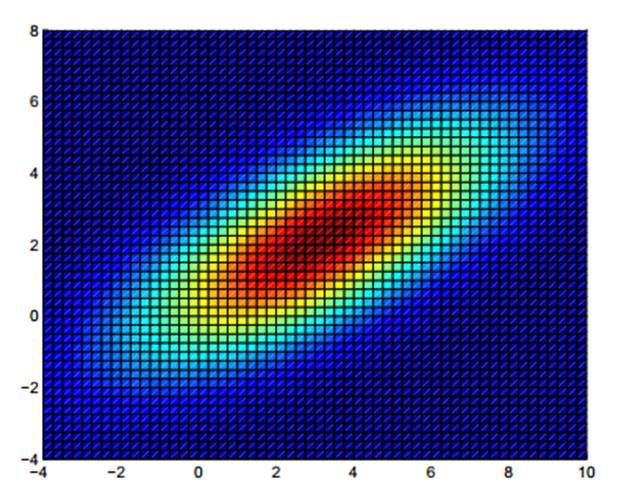
\includegraphics[width=0.8\linewidth]{MVN2}
\end{columns}  
For accurate and efficient MCMC we tune the variance and covariance of the proposal distribution.
\end{frame}

\begin{frame}[label=sec-8-3a]{Why I like hairy caterpillars}
  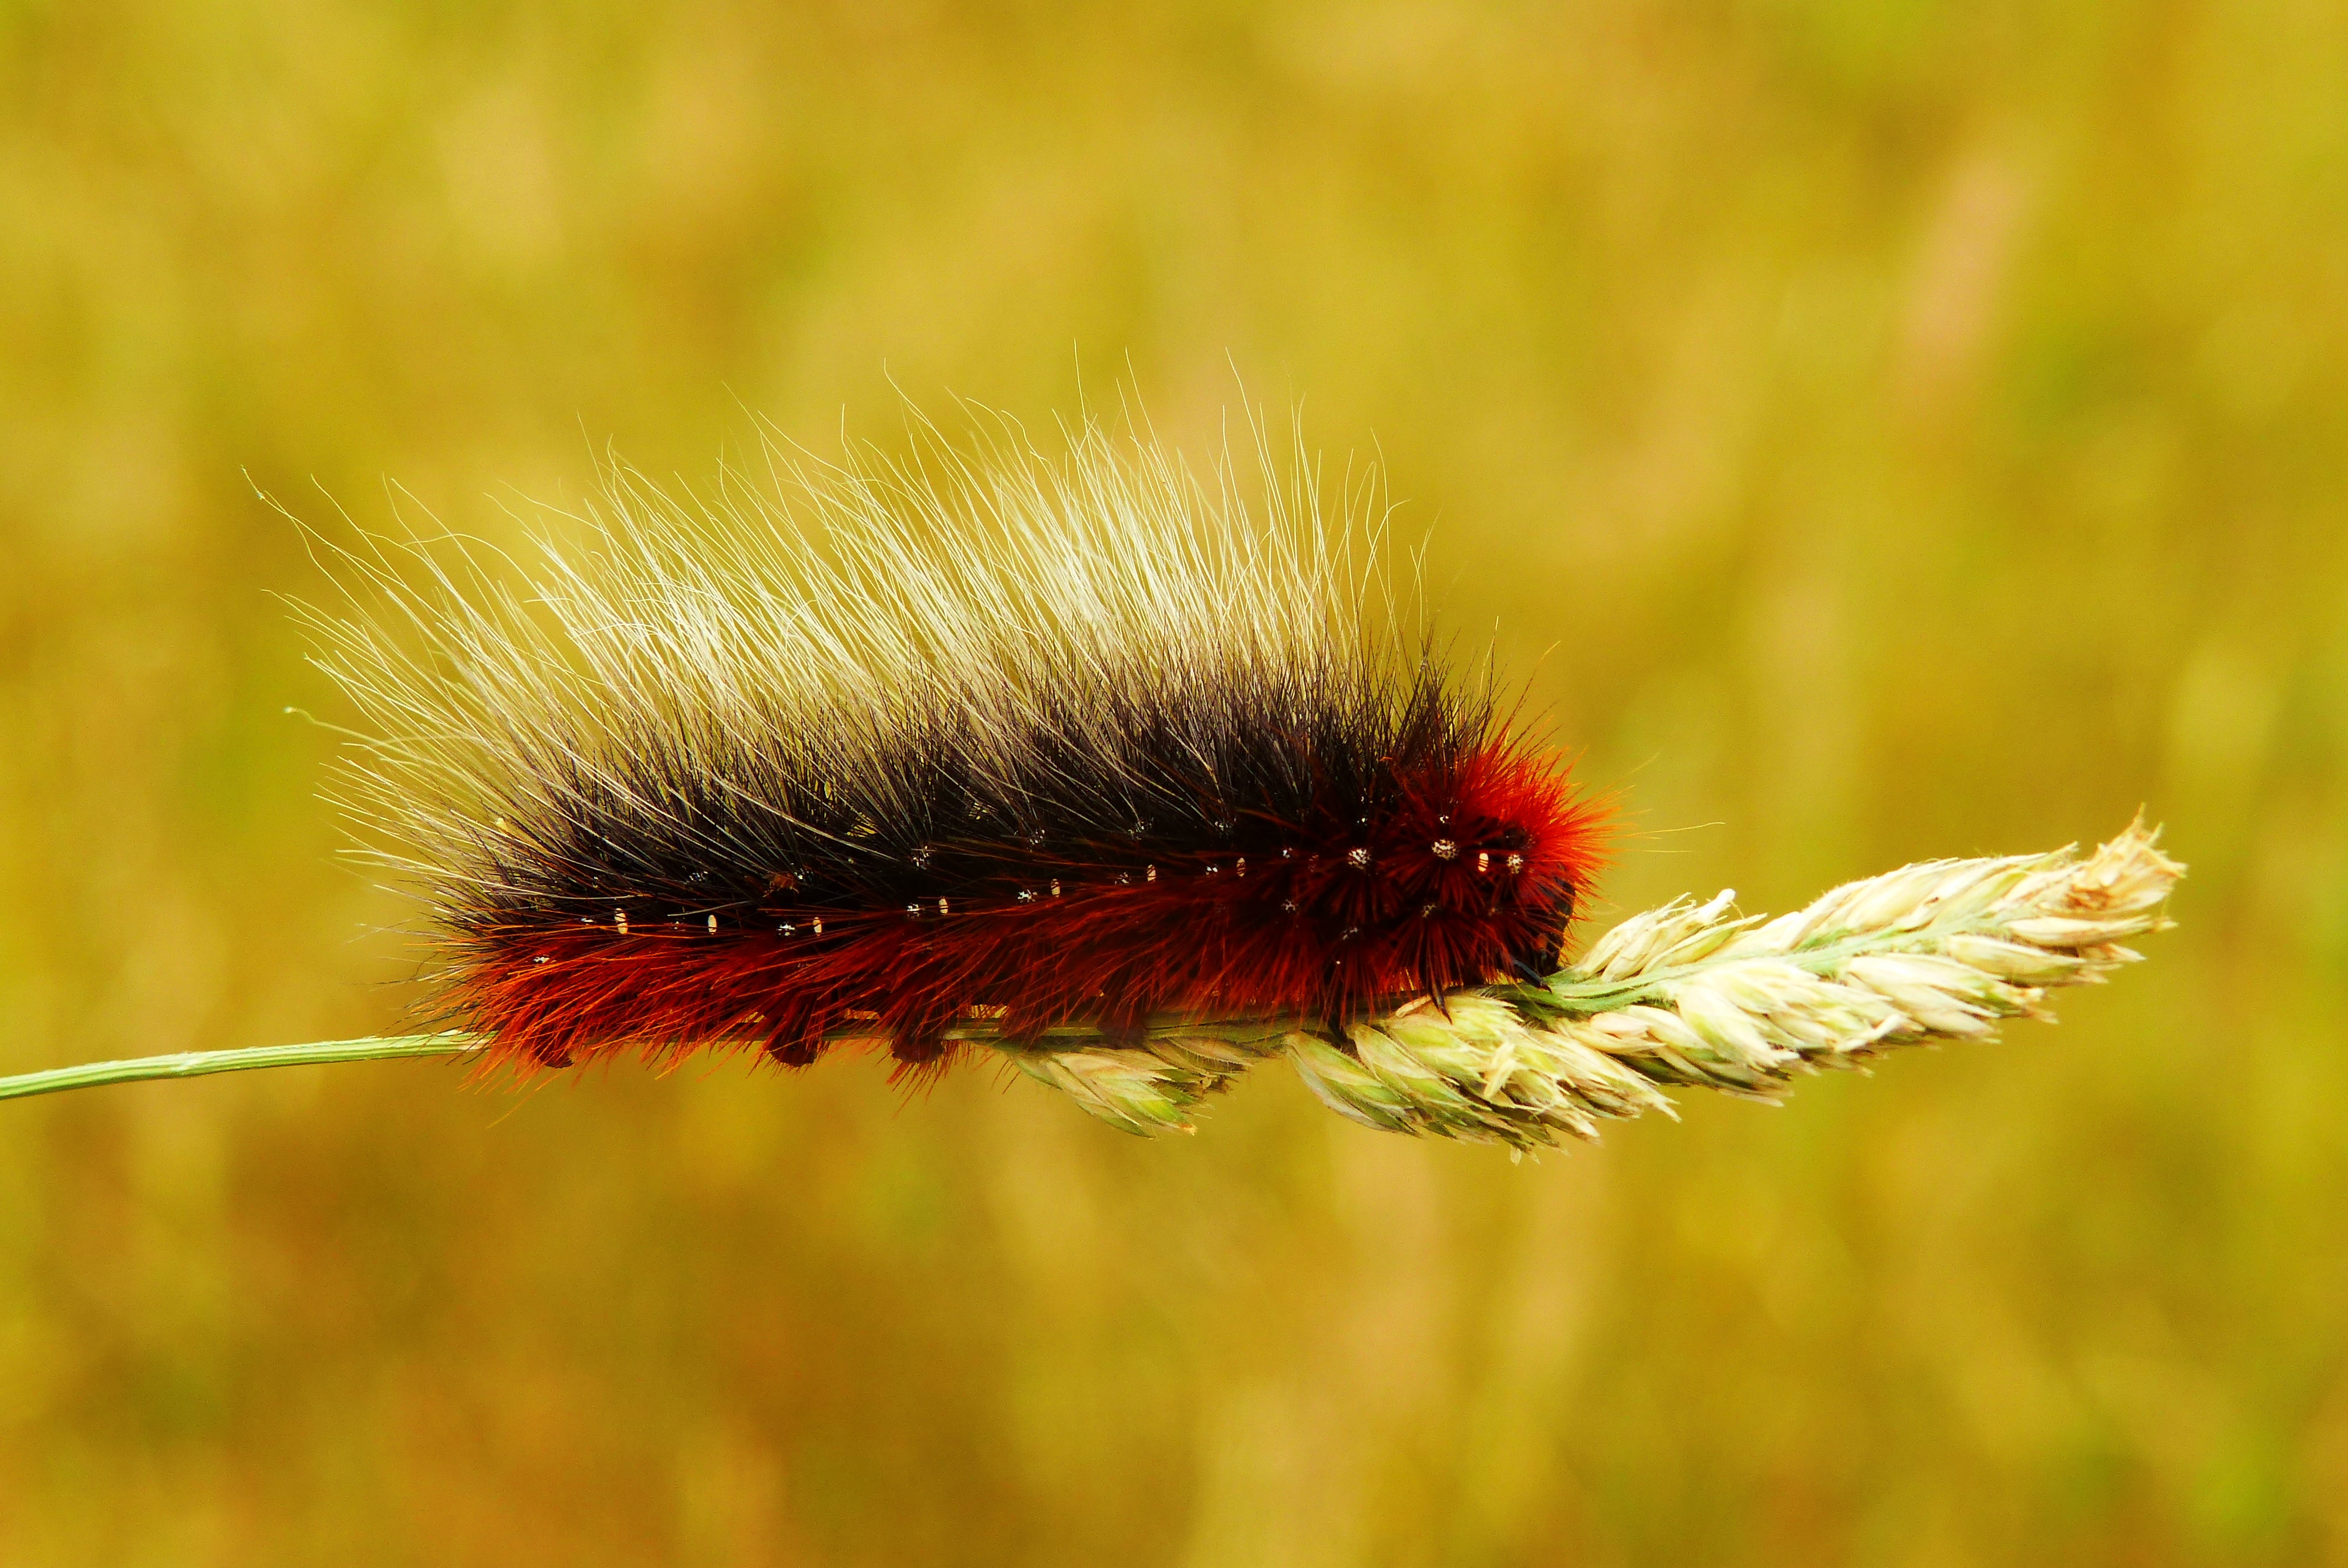
\includegraphics[width=0.7\linewidth]{hairy_catapillar_1.jpg}\\
  Key characterisitics
  \begin{itemize}
    \item Straight
    \item Plump head, plump rear!
    \item Multiple colours
  \end{itemize}
\end{frame}

\begin{frame}[label=sec-8-3]{Choosing a proposal distribution}
    If \alert {variance is too small}, the chain will be slow to reach the target distribution.
    \begin{columns}[c] 
    \column{.5\textwidth} 
    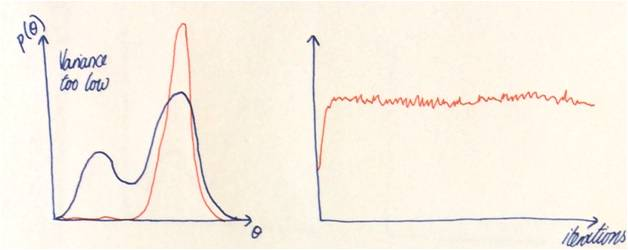
\includegraphics[width=0.8\linewidth]{Var1}
    \column{.5\textwidth}
    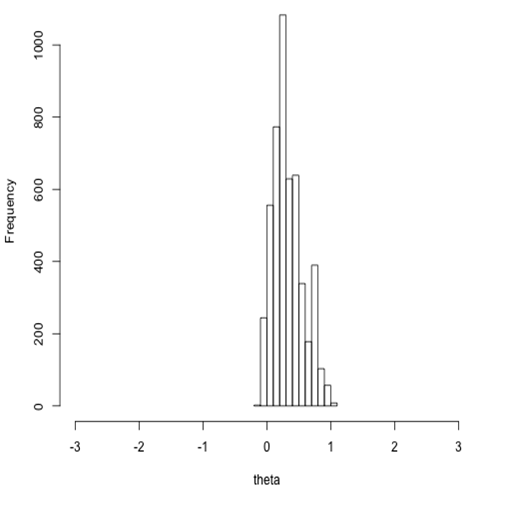
\includegraphics[width=0.8\linewidth]{Trace1}
\end{columns}  
\end{frame}

\begin{frame}[label=sec-8-4]{Choosing a proposal distribution}
    If \alert{variance is too high}, many proposed values will be rejected and the chain will \textit{stick} in one place for many steps.
    \begin{columns}[c] 
    \column{.5\textwidth} 
    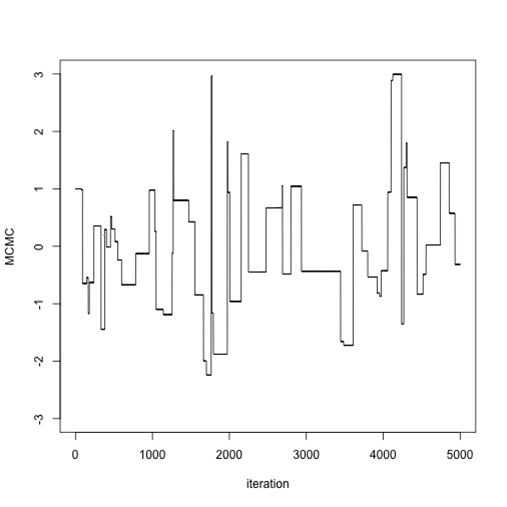
\includegraphics[width=0.8\linewidth]{Var2}
    \column{.5\textwidth}
    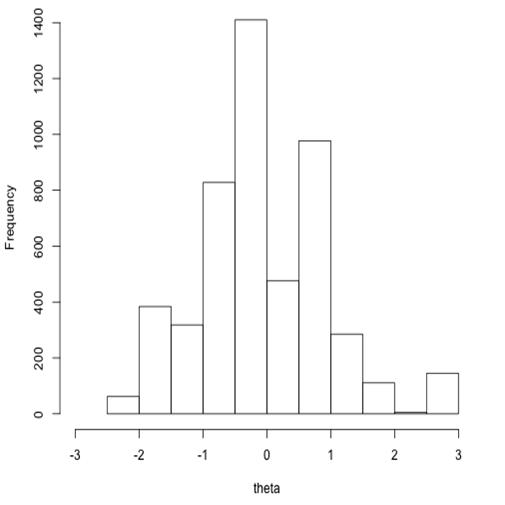
\includegraphics[width=0.8\linewidth]{Trace2}
\end{columns}  
\end{frame}

\begin{frame}[label=sec-8-5]{Choosing a proposal distribution}
    If \alert{variance is just right}, the chain will efficiently explore the full shape of the target distribution.
    \begin{columns}[c] 
    \column{.5\textwidth} 
    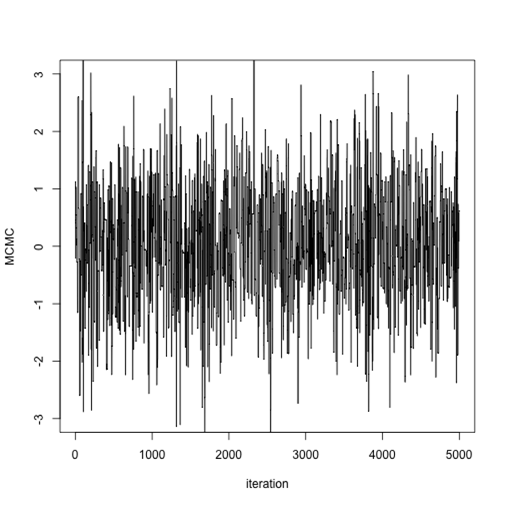
\includegraphics[width=0.8\linewidth]{Var3}
    \column{.5\textwidth}
    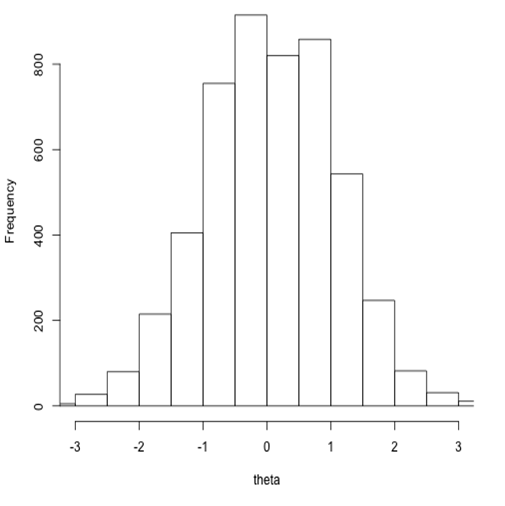
\includegraphics[width=0.8\linewidth]{Trace3}
\end{columns}  
Try several different proposal distributions (\alert{pilot runs}), aiming for an acceptance rate between 24\%  and 40\%. 
\end{frame}

\begin{frame}[label=sec-8-6]{Adaptive MCMC}
    \begin{itemize}
        \item \alert{Adaptive MCMC} alters proposal distribution while chain is running. \\~\\
        \item Start with large symmetric variance, scan around to find a mode. \\~\\
        \item Then alter shape of proposal distribution to match covariance matrix of accepted values.\\~\\
        \item Eventually proposal density should match the shape of target density.\\~\\
    \end{itemize}
\end{frame}

\begin{frame}[label=sec-8-7]{Adaptive MCMC}
    Two-stage adaptation
    \begin{columns}[c] 
    \column{.5\textwidth} 
    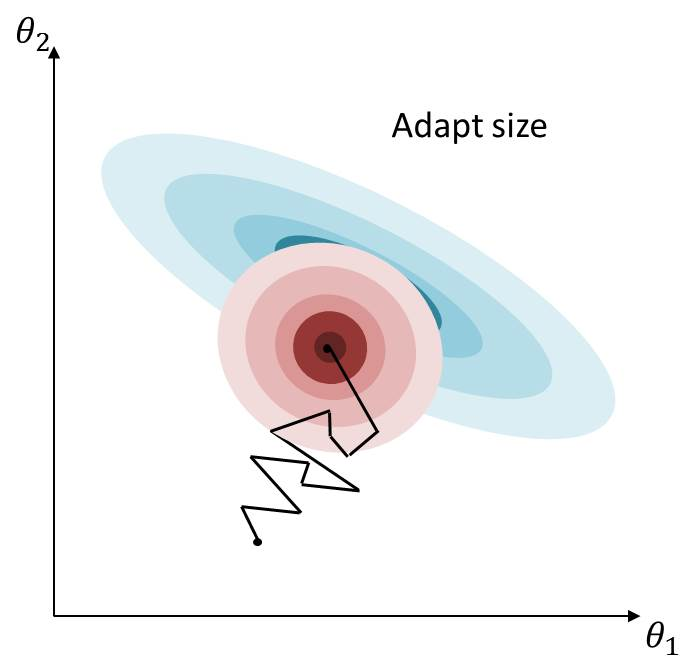
\includegraphics[width=.8\linewidth]{MH7.jpg}
    \column{.5\textwidth} 
    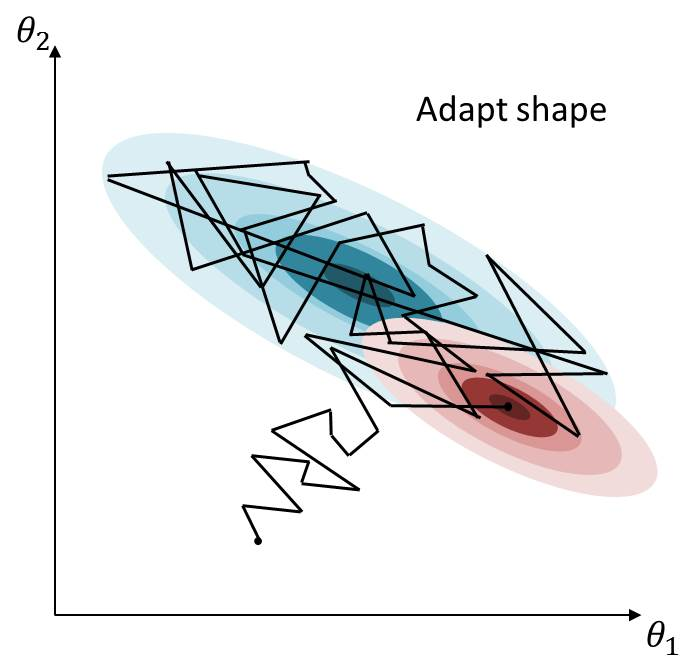
\includegraphics[width=.8\linewidth]{MH8.jpg}
\end{columns}
\end{frame}

\begin{frame}[label=sec-8-8]{Burn-in}
    \begin{columns}[c] 
    \column{.6\textwidth} 
    \begin{itemize}
        \item We can start our MCMC chain anywhere. \\~\\
        \item It can take a while to reach and explore the target density $f(\theta)$. \\~\\
        \item Throw away early samples: \alert{burn-in} phase. \\~\\
        \item How much to discard? \\~\\
    \end{itemize}
    \column{.5\textwidth} 
    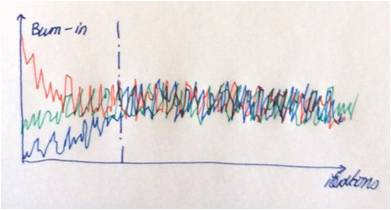
\includegraphics[width=0.75\linewidth]{Burn}
    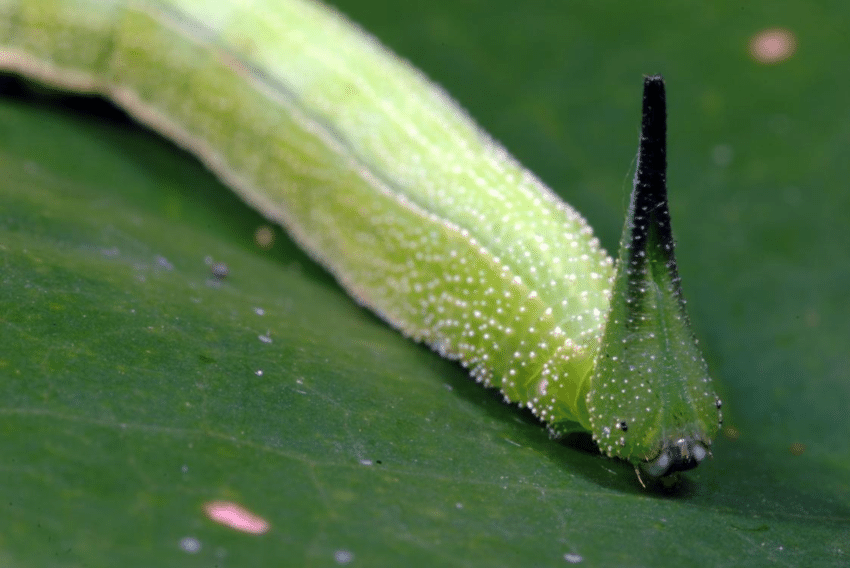
\includegraphics[width=0.75\linewidth]{Hairy-caterpillar-Lepidoptera.png}
    \emph{Lepidoptera} caterpillar
\end{columns}
\end{frame} 

\begin{frame}[label=sec-8-9]{MCMC sample size}
    \begin{itemize}
        \item In MCMC, each sample depends on the one before - \alert{auto-correlation} \\~\\
        \item Reduce degree of auto-correlation by \alert{thinning}, only retain every $n^{th}$ sample. \\~\\
        \item Information content of MCMC samples is given by the \alert{effective sample size (ESS)}. \\~\\
        \item We use the R package \textit{coda}.
    \end{itemize}
\end{frame}

\begin{frame}[label=sec-8-10]{Accuracy and efficiency}
  How does each element influence accuracy and efficiency?
  \begin{itemize}
    \item Burn-in
    \item MCMC iterations (after burn-in)
    \item Thinning
    \item Number of chains (with different initial conditions)
    \item Proposal distribution
    \item Transforming parameters
  \end{itemize}
\end{frame}


\end{document}
